\documentclass[a4paper,11pt]{article}
\usepackage{amsmath,amsthm,amsfonts,amssymb,amscd,amstext,vmargin,graphics,graphicx,tabularx,multicol} \usepackage[french]{babel}
\usepackage[utf8]{inputenc}  
\usepackage[T1]{fontenc} 
\usepackage[T1]{fontenc}
\usepackage{amsmath,amssymb}
\usepackage{pstricks-add,tikz,tkz-tab,variations}
\usepackage[autolanguage,np]{numprint} 
\usepackage{color}
\usepackage{ulem}

\setmarginsrb{1.5cm}{0.5cm}{1cm}{0.5cm}{0cm}{0cm}{0cm}{0cm} %Gauche, haut, droite, haut
\newcounter{numexo}
\newcommand{\exo}[1]{\stepcounter{numexo}\noindent{\bf Exercice~\thenumexo} : \marginpar{\hfill /#1}}
\reversemarginpar


\newcounter{enumtabi}
\newcounter{enumtaba}
\newcommand{\q}{\stepcounter{enumtabi} \theenumtabi.  }
\newcommand{\qa}{\stepcounter{enumtaba} (\alph{enumtaba}) }
\newcommand{\initq}{\setcounter{enumtabi}{0}}
\newcommand{\initqa}{\setcounter{enumtaba}{0}}

\newcommand{\be}{\begin{enumerate}}
\newcommand{\ee}{\end{enumerate}}
\newcommand{\bi}{\begin{itemize}}
\newcommand{\ei}{\end{itemize}}
\newcommand{\bp}{\begin{pspicture*}}
\newcommand{\ep}{\end{pspicture*}}
\newcommand{\bt}{\begin{tabular}}
\newcommand{\et}{\end{tabular}}
\renewcommand{\tabularxcolumn}[1]{>{\centering}m{#1}} %(colonne m{} centrée, au lieu de p par défault) 
\newcommand{\tnl}{\tabularnewline}

\newcommand{\trait}{\noindent \rule{\linewidth}{0.2mm}}
\newcommand{\hs}[1]{\hspace{#1}}
\newcommand{\vs}[1]{\vspace{#1}}

\newcommand{\N}{\mathbb{N}}
\newcommand{\Z}{\mathbb{Z}}
\newcommand{\R}{\mathbb{R}}
\newcommand{\C}{\mathbb{C}}
\newcommand{\Dcal}{\mathcal{D}}
\newcommand{\Ccal}{\mathcal{C}}
\newcommand{\mc}{\mathcal}

\newcommand{\vect}[1]{\overrightarrow{#1}}
\newcommand{\ds}{\displaystyle}
\newcommand{\eq}{\quad \Leftrightarrow \quad}
\newcommand{\vecti}{\vec{\imath}}
\newcommand{\vectj}{\vec{\jmath}}
\newcommand{\Oij}{(O;\vec{\imath}, \vec{\jmath})}
\newcommand{\OIJ}{(O;I,J)}

\newcommand{\bmul}[1]{\begin{multicols}{#1}}
\newcommand{\emul}{\end{multicols}}


\newcommand{\reponse}[1][1]{%
\multido{}{#1}{\makebox[\linewidth]{\rule[0pt]{0pt}{20pt}\dotfill}
}}

\newcommand{\titre}[5] 
% #1: titre #2: haut gauche #3: bas gauche #4: haut droite #5: bas droite
{
\noindent #2 \hfill #4 \\
#3 \hfill #5

\vspace{-1.6cm}

\begin{center}\rule{6cm}{0.5mm}\end{center}
\vspace{0.2cm}
\begin{center}{\large{\textbf{#1}}}\end{center}
\begin{center}\rule{6cm}{0.5mm}\end{center}
}



\begin{document}
\pagestyle{empty}
\titre{Interrogation : Notions de fonctions}{Nom :}{Prénom :}{Date}{Classe}


\vspace*{0.5cm}

\exo{3} Soit $f$ la fonction définie par $f(x) = -3x^{2}+2x-5$.\\

\q Compléter :

\bmul{2}

$f(0)= . . .$ \\

\columnbreak

$f(-1)= . . .$ \\

\emul

\q Quelle est l'image de 2 par la fonction $f$? \\
\reponse[1]\\

\q Quel est l'antécédent de - 5 par la fonction $f$ ?\\
\reponse[1]\\

\vspace*{0.5cm}


\exo{5} La fonction $f$ est représentée par la courbe représentative $C_{f}$ ci-dessous.\\

\begin{center}
\includegraphics[scale=0.7]{courbeinterro1.eps} 
\end{center}


\initq \q Quelle est l'image de - 3 par la fonction f ?\\
\reponse[1]\\

\q	Quelle est l'image de 2 par la fonction f ?\\
\reponse[1]\\

\q	Donner les antécédents de – 1 par la fonction f ?\\
\reponse[1]\\

\q	Quel nombre a pour antécédent 0 par la fonction f ?\\
\reponse[1]\\

\q	Quel(s) nombre(s) ont pour image 0 par la fonction f ?\\
\reponse[1]\\

\q	Compléter les égalités :\\

$f(-6) = . . .$ \hspace*{0.3cm} $f(. . .) = -3$ \hspace*{0.3cm} $f(4) = . . .$ \hspace*{0.3cm} $f(. . .) = 3$\\


\newpage

\exo{2}
On considère la fonction  $h$ définie par $ h(x) = - 4x^{2} +7$.\\

\initq \q Compléter le tableau de valeurs suivant ( aucune justification n'est attendue ) :



\begin{center}
\begin{tabular}{|c|c|c|c|c|c|}
\hline 
x & \hspace*{0.2cm}-2 \hspace*{0.2cm}& \hspace*{0.2cm} -1\hspace*{0.2cm} & \hspace*{0.2cm}0 \hspace*{0.2cm}& \hspace*{0.2cm} 1 \hspace*{0.2cm}& \hspace*{0.2cm} 2 \hspace*{0.2cm}\\ 
\hline 
$h(x)$ &  &  &  &  &\\ 
\hline 
\end{tabular} 
\end{center}

\vspace*{1cm}

\q Tracer dans le repère ci-dessous une courbe représentant la fonction $h$.\\

\begin{center}

\includegraphics[scale=1]{grille.eps} 
\end{center}




\end{document}
